\section{Техническое задание}

\subsection{Основание для выполнения работы}

Основанием для выполнения работы является учебный план направления
02.03.01 «Математика и компьютерные науки» Высшей школы технологий искусственного интеллекта Института компьютерных наук и кибербезопасности
Санкт-Петербургского Политехнического университета Петра Великого,
который предусматривает выполнение курсовой работы по дисциплине
«Функциональное программирование».

\subsection{Исполнитель и соисполнители работы}

Исполнитель: студент учебной группы 5130201/40101 Резчик Денис Олегович.

\subsection{Цели, задачи и исходные данные}

\subsubsection{Цель работы}

Целью работы является создание рекомендательной системы подбора фильмов на основе анализа описаний фильмов с использованием методов машинного обучения (TF-IDF векторизация и косинусная мера сходства).

\subsubsection{Задачи работы}

\begin{enumerate}
    \item Изучить набор данных Movie Dataset, выбранных для построения модели.
    \item Реализовать модуль загрузки данных из CSV файла (CSVLoader).
    \item Реализовать модуль предобработки текста: токенизация, удаление стоп-слов, нормализация текста.
    \item Реализовать модуль TF-IDF векторизации описаний фильмов.
    \item Обучить модель на основе косинусной меры сходства. Реализовать сохранение векторов и весов в отдельные файлы.
    \item Реализовать консольный интерфейс с двумя способами ввода интересующих пользователя фильмов:
    интерактивный ввод названий фильмов в консоль и загрузка списка фильмов из текстового файла.
    \item Реализовать модуль оценки качества модели (ModelEvaluation) с вычислением метрик сходства.
    \item Реализовать систему логирования действий пользователя и системных событий в текстовый файл.
    \item Обеспечить систему обработки ошибок: отсутствие файлов, неправильный ввод.
    \item Написать набор тестов с использованием QuickCheck.
\end{enumerate}

\subsubsection{Исходные данные}

Исходными данными для выполнения данной работы является набор данных о фильмах <<Movie Dataset>>, опубликованный на платформе Kaggle. Он представляет собой CSV-файл с описанием фильмов. Основные используемые признаки:

\begin{table}[H]
\centering
\begin{tabularx}{\textwidth}{|l|l|X|}
\hline
\textbf{Признак} & \textbf{Тип} & \textbf{Описание} \\
\hline
\texttt{id}  & Int & Уникальный идентификатор фильма \\
\texttt{original\_title} & String & Оригинальное название фильма \\
\texttt{overview} & String & Описание сюжета фильма \\
\texttt{keywords} & [String] & Ключевые слова, характеризующие фильм \\
\texttt{genres} & [String] & Жанры фильма \\
\texttt{popularity} & Double & Метрика популярности фильма \\
\hline
\end{tabularx}
\label{features}
\caption{Описание основных признаков датасета}
\end{table}

\subsection{Основное содержание работы}

Приложение представляет собой консольную систему рекомендаций фильмов, построенную на основе TF-IDF векторизации описаний фильмов и вычисления косинусной меры сходства между ними.

\subsubsection{Модули приложения}

\begin{enumerate}
    \item CSVLoader --- загружает данные из CSV файла, сохраняет информацию о фильмах в структурированном виде.
    
    \item Preprocessing --- модуль обработки текста: преобразование регистра, удаление пунктуации, удаление стоп-слов для подготовки текста к анализу моделью.
    
    \item TFIDFVectorizer --- построение словаря из описаний фильмов, вычисление TF-IDF векторов для каждого фильма с использованием sparse представления.
    
    \item Recommender --- поиск подходящих фильмов с помощью косинусной меры сходства между TF-IDF векторами.
    
    \item ModelEvaluation --- вычисление метрик качества модели: схожесть описаний фильмов одного жанра, разреженность векторов, покрытие датасета.
    
    \item ModelPersistence --- кеширование предобученной модели. Сохраняет словарь, IDF-веса и TF-IDF профили фильмов в CSV-файлы для быстрой загрузки при последующих запусках.
    
    \item Logger --- логирование основных операций системы в файл app.log: загрузка данных, построение модели, запросы пользователя, ошибки.
    
    \item UI --- интерактивное меню, ввод параметров, обработка неправильного ввода информации, вывод результатов рекомендаций в консоль.
\end{enumerate}

\subsection{Основные требования к выполнению работы}

\subsubsection{Назначение разрабатываемого программного комплекса}

Разрабатываемый программный комплекс предназначен для рекомендации фильмов на основе анализа их описаний. Пользователь выбирает интересующие его фильмы, а система находит и рекомендует похожие фильмы, используя методы векторизации текста и вычисления мер сходства.

\subsection{Технические характеристики по назначению}

Программное обеспечение должно обеспечить следующие технические характеристики:

\begin{enumerate}
    \item Среднее косинусное сходство между фильмами одного жанра на валидационной выборке 
    — не менее 0,3 (30\%).
    
    \item Время загрузки датасета и построения модели TF-IDF на первый запуск — 
    не более 5 минут на стандартном персональном компьютере.
    
    \item Время загрузки кешированной модели (словарь, IDF-веса, векторы) при повторных запусках — 
    не более 2 секунд.
    
    \item Время обработки запроса пользователя (поиск рекомендаций для 1-5 выбранных фильмов) — 
    не более 10 секунд.
    
    \item Размер кешированной модели (CSV-файлы) — не более 500 МБ.
    
    \item Покрытие датасета (процент успешно обработанных фильмов) — не менее 95\%.
\end{enumerate}

\subsubsection{Функциональные требования}

\subsubsection*{Загрузка и предобработка данных}

\begin{enumerate}
    \item Приложение должно читать CSV файл с данными о фильмах.
    \item Для каждого фильма извлечь: ID, название, описание (overview), ключевые слова.
    \item Применить Preprocessing: нормализация регистра, удаление пунктуации, токенизация, удаление стоп-слов.
    \item Результаты предобработки должны использоваться для построения TF-IDF модели.
\end{enumerate}

\subsubsection*{Обучение модели}

\begin{enumerate}
    \item Датасет делится на обучающую (70\%), валидационную (15\%) и тестовую (15\%) выборки.
    
    \item На обучающей выборке:
    \begin{itemize}
        \item Строится словарь (Vocabulary) из уникальных слов.
        \item Вычисляются значения IDF (Inverse Document Frequency) для каждого слова.
    \end{itemize}
    
    \item На валидационной выборке:
    \begin{itemize}
        \item Вычисляются TF-IDF векторы для фильмов.
        \item Вычисляются метрики внутригруппового сходства (intra-film similarity).
        \item Проверяется адекватность разреженности векторов.
    \end{itemize}
    
    \item На тестовой выборке:
    \begin{itemize}
        \item Вычисляются TF-IDF векторы.
        \item Проводится итоговая оценка качества модели.
        \item Вычисляются метрики: среднее сходство, покрытие датасета, разреженность векторов.
    \end{itemize}
    
    \item Предобработка текстовых признаков: нормализация регистра, удаление пунктуации, 
    токенизация, удаление стоп-слов.
    
    \item Построенная модель (словарь, IDF-веса, TF-IDF векторы фильмов) сохраняется 
    в CSV-файлы для дальнейшей загрузки при использовании приложения.
\end{enumerate}

\subsubsection*{Рекомендация фильмов}

\begin{enumerate}
    \item Пользователь выбирает один или несколько фильмов по названию.
    \item Система вычисляет средний TF-IDF вектор выбранных фильмов.
    \item Для каждого остального фильма вычисляется косинусная мера сходства с вектором пользователя.
    \item Система сортирует фильмы по значению косинусной меры в убывающем порядке.
    \item Выводит топ-10 рекомендованных фильмов с указанием оценки сходства (0-100\%).
\end{enumerate}

\subsubsection*{Оценка качества модели}

\begin{enumerate}
    \item Вычислить среднее внутригруппповое сходство (для фильмов одного жанра).
    \item Вычислить среднюю разреженность векторов.
    \item Вычислить покрытие датасета (процент обработанных фильмов).
    \item Вывести метрики на экран при запуске.
\end{enumerate}

\subsubsection*{Обработка ошибок и логирование}

\begin{enumerate}
    \item Обработка некорректного ввода пользователя (пустой текст, несуществующие ID).
    \item Обработка отсутствия файлов (CSV, кешированная модель).
    \item Вывод понятных сообщений об ошибках.
    \item Все действия должны логироваться в app.log с временными метками.
\end{enumerate}

\subsection{Этапы и сроки выполнения работы}

\subsubsection{Перечень этапов}

\begin{enumerate}
    \item Этап 1. Выбор датасета и составление технического задания (до 08.09.2026).
    \\ Выбор Movie Dataset, анализ структуры, разработка технического задания.
    
    \item Этап 2. Проектирование архитектуры (до 09.09.2026).
    \\ Диаграмма типов и модулей, описание структур данных, обоснование выбора библиотек.
    
    \item Этап 3. Разработка загрузки данных и предобработки текста (до 10.09.2026).
    \\ Реализация CSVLoader, Preprocessing модулей.
    
    \item Этап 4. Разработка TF-IDF и оценка качества (до 10.09.2026).
    \\ Реализация TFIDFVectorizer и ModelEvaluation модулей.
    
    \item Этап 5. Реализация рекомендаций и сохранения модели (до 11.09.2026).
    \\ Реализация Recommender и ModelPersistence модулей.
    
    \item Этап 6. Разработка UI и логирования (до 11.09.2026).
    \\ Реализация UI и Logger модулей, интеграция компонентов.
    
    \item Этап 7. Тестирование и документация (до 12.09.2026).
    \\ Написание тестов QuickCheck, разработка документации.
\end{enumerate}

\subsubsection{Диаграмма Ганта}

\begin{figure}[H]
    \centering
    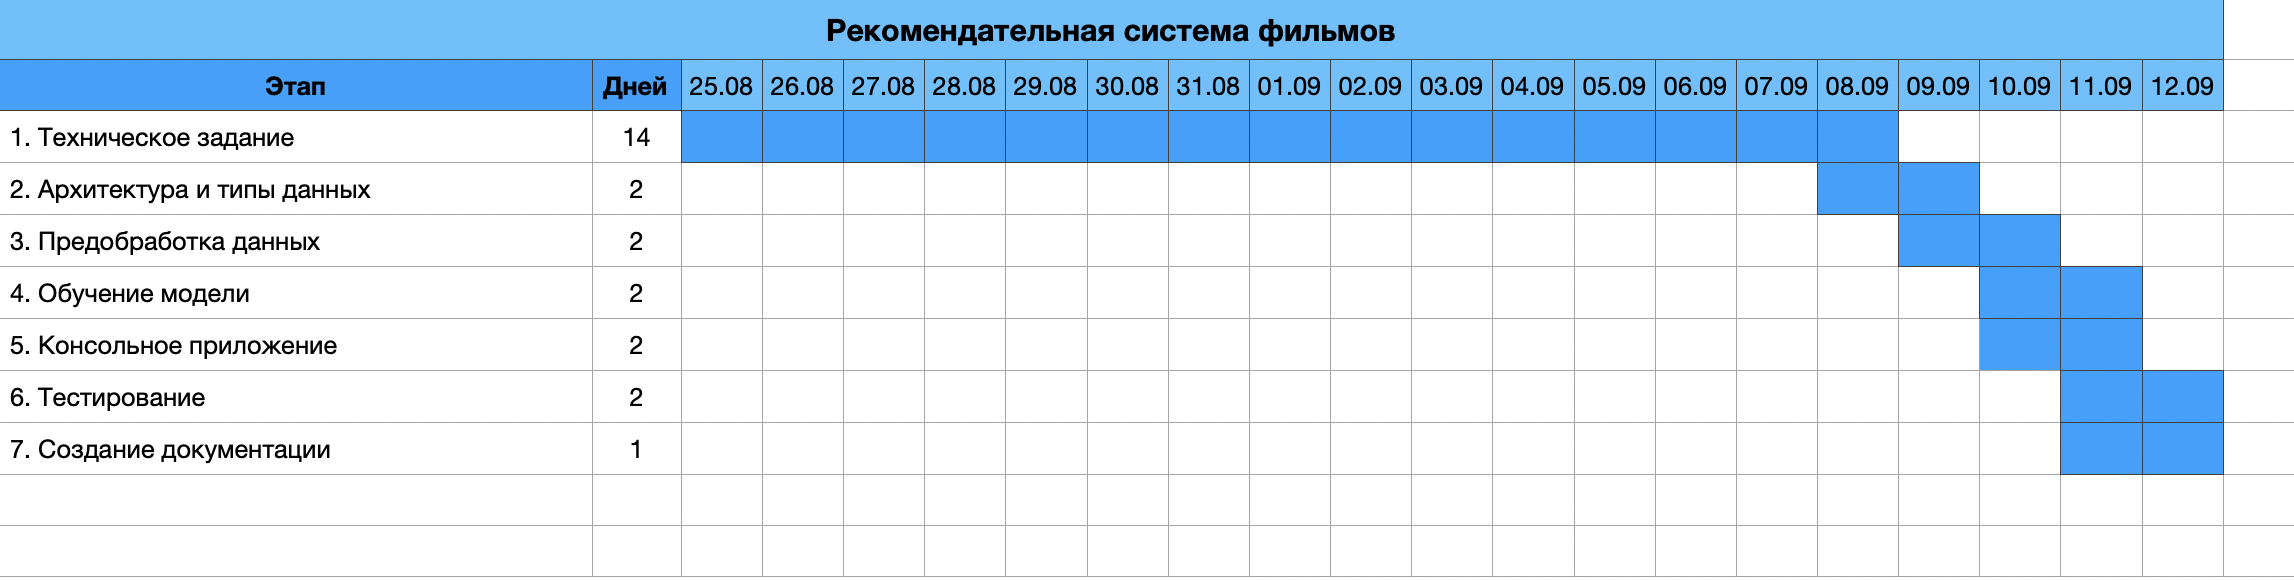
\includegraphics[height=5cm]{Gant.png}
    \caption{Диаграмма Ганта}
\end{figure}    

\subsection{Результаты работы}

\begin{enumerate}
    \item Согласованное техническое задание.
    
    \item Описание архитектуры проекта: диаграмма типов и модулей, описание структур данных.
    
    \item Работающие модули обработки данных: CSVLoader, Preprocessing, TFIDFVectorizer.
    
    \item Модуль оценки качества модели (ModelEvaluation) с вычисленными метриками.
    
    \item Модуль сохранения и загрузки модели (ModelPersistence) с поддержкой кеширования.
    
    \item Работающее консольное приложение movie-recommender с возможностью получения рекомендаций по заданным фильмам.
    
    \item Система логирования с записью всех событий в app.log.
    
    \item Набор тестов QuickCheck для проверки корректности основных функций.
    
    \item Отчёт о выполненной курсовой работе с описанием выполнения работы и результатов.
\end{enumerate}